\documentclass[11pt]{article}

\usepackage[utf8]{inputenc}
\usepackage{geometry}
\geometry{a4paper}
\usepackage{graphicx}
\usepackage{booktabs}
\usepackage{array}
\usepackage{verbatim}
\usepackage{subfig}
\usepackage{hyperref}

\usepackage{url}

\usepackage{fancyhdr} 
\pagestyle{fancy}
\renewcommand{\headrulewidth}{0pt} 
\lhead{}\chead{}\rhead{}
\lfoot{}\cfoot{\thepage}\rfoot{}

\usepackage{sectsty}
\allsectionsfont{\sffamily\mdseries\upshape}

\usepackage[nottoc,notlof,notlot]{tocbibind} 
\usepackage[titles,subfigure]{tocloft} 
\renewcommand{\cftsecfont}{\rmfamily\mdseries\upshape}
\renewcommand{\cftsecpagefont}{\rmfamily\mdseries\upshape}

\usepackage[spanish]{babel}
\usepackage{listings}

%%%El documento comienza aqui

\title{\textbf{Proyecto de Parseo de Archivos XML - Lenguaje Python}}
\author{\textbf{Jose Luis Bueno - Erick Buendia}}
\date{\textbf{\today}}
\begin{document}

\bibliographystyle{plain}

\maketitle
\section{\textbf{Introducción}} 
\paragraph{} \noindent
Este proyecto consiste en leer un archivo tipo XML con unos poco niveles de anidacion y sus datos modelarlos a objetos, y usar las magnificas herramientas que nos ofrece este gran lenguaje de programacion.\newline
Las ventajas que nos ofrece este lenguaje son muchas, la principal es el manejo de cadenas de caracteres, fuerte tipado de tipos y entre otras.
\section{\textbf{Alcance del Proyecto}}

El proyecto logro los objetivos siguientes:
\begin{enumerate}
\item 
Lectura de los atributos y tags del archivo XML.

\item
Clases y metodos modulados.

\item
Todos los tags se convirtieron en una clase para su mejor manejo.
\end{enumerate}

\section{\textbf{Diagramación}}


\subsection{\textbf{Diagrama UML de los tags}}

				\begin{center}
				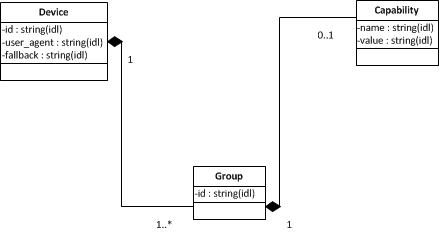
\includegraphics[width=0.71\textwidth]{images/diagrama}
				\end{center}

\section{\textbf{Conclusiones}}
\begin{enumerate}
\item
El lenguaje de programación Python ofrece una buena administracion de memoria gracias a su buen garbage collector.
\item
Tambien ofrece mucha ayuda en el manejo de cadenas de caracteres, tarea que en otros lenguajes resulta muy compleja.
\item
Es sin duda el lenguaje de programacion con un nivel de aprendizaje mas intuitivo.
\item
Este proyecto se desarrollo con la version 2.7 y el IDE usado fue Geany
\end{enumerate}

\section{\textbf{Recomendaciones}}
\begin{enumerate}
\item
Se observaron diferencias considerables entre Python 2.7 y Python 3.3, lo cual cierto codigo de una version no es completamente compatible con la otra
\item
Para encapsular los atributos de las clases se antepone el doble subguion antes del nombre
\item
Consultar la guia de referencia del lenguaje en la pagina oficial de Python

\end{enumerate}


\end{document}